\documentclass{article}
\usepackage[paperwidth=215.9mm,paperheight=279.4mm,margin=0mm]{geometry}
\usepackage[T1]{fontenc}
\usepackage{helvet}
\renewcommand{\familydefault}{\sfdefault}
\usepackage{tikz}
\usetikzlibrary{arrows.meta}
\pagestyle{empty}
\setlength{\parindent}{0pt}
\ifdefined\pdfinfoomitdate\pdfinfoomitdate=1\fi
\ifdefined\pdftrailerid\pdftrailerid{}\fi
\ifdefined\pdfsuppressptexinfo\pdfsuppressptexinfo=15\fi
\begin{document}
\null\begin{tikzpicture}[remember picture,overlay,x=1mm,y=-1mm]
\begin{scope}[shift={(current page.north west)}]
\node[anchor=north west,inner sep=0pt,align=left,font=\fontsize{10}{12.2}\selectfont] at (10,6) {Week 35 / Footprint borders / Materials};
\draw[line width=.5pt] (10,11.5) -- (205.9,11.5);
\node[anchor=north west,inner sep=0pt,align=left,text width=195.9mm,font=\fontsize{10.5}{12.8}\selectfont] at (10,14) {\textbf{Footprint cards. Print 1 per table on card stock.} Each set is 24 cards for one pair or trio: 12 A cards and 12 mirror-A cards. A table with one group can start with Set 1 only. Cut on the lines.};
\draw[line width=.8pt] (10,27) -- (110,27);
\draw[line width=.8pt] (10,25) -- (10,29);
\draw[line width=.8pt] (110,25) -- (110,29);
\node[anchor=west,inner sep=0pt,align=left,font=\fontsize{8}{9.8}\selectfont] at (113,27) {10 cm scale check: measure before cutting};
\node[anchor=south west,inner sep=0pt,align=left,font=\fontsize{9}{11.0}\selectfont] at (20.95,36.5) {Set 1: two rows of A, then two rows of mirror A};
\draw[line width=.5pt] (20.95,38) rectangle (49.95,64);
\draw[line width=.7pt,fill=black!15] (22.45,40) -- (48.45,40) -- (48.45,47) -- (43.45,47) -- (43.45,44.5) -- (30.45,44.5) -- (30.45,51) -- (41.45,51) -- (41.45,55.5) -- (30.45,55.5) -- (30.45,62) -- (22.45,62) -- cycle;
\draw[-{Stealth},line width=.65pt] (32.95,42.4) -- (40.95,42.4);
\draw[line width=.5pt] (49.95,38) rectangle (78.95,64);
\draw[line width=.7pt,fill=black!15] (51.45,40) -- (77.45,40) -- (77.45,47) -- (72.45,47) -- (72.45,44.5) -- (59.45,44.5) -- (59.45,51) -- (70.45,51) -- (70.45,55.5) -- (59.45,55.5) -- (59.45,62) -- (51.45,62) -- cycle;
\draw[-{Stealth},line width=.65pt] (61.95,42.4) -- (69.95,42.4);
\draw[line width=.5pt] (78.95,38) rectangle (107.95,64);
\draw[line width=.7pt,fill=black!15] (80.45,40) -- (106.45,40) -- (106.45,47) -- (101.45,47) -- (101.45,44.5) -- (88.45,44.5) -- (88.45,51) -- (99.45,51) -- (99.45,55.5) -- (88.45,55.5) -- (88.45,62) -- (80.45,62) -- cycle;
\draw[-{Stealth},line width=.65pt] (90.95,42.4) -- (98.95,42.4);
\draw[line width=.5pt] (107.95,38) rectangle (136.95,64);
\draw[line width=.7pt,fill=black!15] (109.45,40) -- (135.45,40) -- (135.45,47) -- (130.45,47) -- (130.45,44.5) -- (117.45,44.5) -- (117.45,51) -- (128.45,51) -- (128.45,55.5) -- (117.45,55.5) -- (117.45,62) -- (109.45,62) -- cycle;
\draw[-{Stealth},line width=.65pt] (119.95,42.4) -- (127.95,42.4);
\draw[line width=.5pt] (136.95,38) rectangle (165.95,64);
\draw[line width=.7pt,fill=black!15] (138.45,40) -- (164.45,40) -- (164.45,47) -- (159.45,47) -- (159.45,44.5) -- (146.45,44.5) -- (146.45,51) -- (157.45,51) -- (157.45,55.5) -- (146.45,55.5) -- (146.45,62) -- (138.45,62) -- cycle;
\draw[-{Stealth},line width=.65pt] (148.95,42.4) -- (156.95,42.4);
\draw[line width=.5pt] (165.95,38) rectangle (194.95,64);
\draw[line width=.7pt,fill=black!15] (167.45,40) -- (193.45,40) -- (193.45,47) -- (188.45,47) -- (188.45,44.5) -- (175.45,44.5) -- (175.45,51) -- (186.45,51) -- (186.45,55.5) -- (175.45,55.5) -- (175.45,62) -- (167.45,62) -- cycle;
\draw[-{Stealth},line width=.65pt] (177.95,42.4) -- (185.95,42.4);
\draw[line width=.5pt] (20.95,64) rectangle (49.95,90);
\draw[line width=.7pt,fill=black!15] (22.45,66) -- (48.45,66) -- (48.45,73) -- (43.45,73) -- (43.45,70.5) -- (30.45,70.5) -- (30.45,77) -- (41.45,77) -- (41.45,81.5) -- (30.45,81.5) -- (30.45,88) -- (22.45,88) -- cycle;
\draw[-{Stealth},line width=.65pt] (32.95,68.4) -- (40.95,68.4);
\draw[line width=.5pt] (49.95,64) rectangle (78.95,90);
\draw[line width=.7pt,fill=black!15] (51.45,66) -- (77.45,66) -- (77.45,73) -- (72.45,73) -- (72.45,70.5) -- (59.45,70.5) -- (59.45,77) -- (70.45,77) -- (70.45,81.5) -- (59.45,81.5) -- (59.45,88) -- (51.45,88) -- cycle;
\draw[-{Stealth},line width=.65pt] (61.95,68.4) -- (69.95,68.4);
\draw[line width=.5pt] (78.95,64) rectangle (107.95,90);
\draw[line width=.7pt,fill=black!15] (80.45,66) -- (106.45,66) -- (106.45,73) -- (101.45,73) -- (101.45,70.5) -- (88.45,70.5) -- (88.45,77) -- (99.45,77) -- (99.45,81.5) -- (88.45,81.5) -- (88.45,88) -- (80.45,88) -- cycle;
\draw[-{Stealth},line width=.65pt] (90.95,68.4) -- (98.95,68.4);
\draw[line width=.5pt] (107.95,64) rectangle (136.95,90);
\draw[line width=.7pt,fill=black!15] (109.45,66) -- (135.45,66) -- (135.45,73) -- (130.45,73) -- (130.45,70.5) -- (117.45,70.5) -- (117.45,77) -- (128.45,77) -- (128.45,81.5) -- (117.45,81.5) -- (117.45,88) -- (109.45,88) -- cycle;
\draw[-{Stealth},line width=.65pt] (119.95,68.4) -- (127.95,68.4);
\draw[line width=.5pt] (136.95,64) rectangle (165.95,90);
\draw[line width=.7pt,fill=black!15] (138.45,66) -- (164.45,66) -- (164.45,73) -- (159.45,73) -- (159.45,70.5) -- (146.45,70.5) -- (146.45,77) -- (157.45,77) -- (157.45,81.5) -- (146.45,81.5) -- (146.45,88) -- (138.45,88) -- cycle;
\draw[-{Stealth},line width=.65pt] (148.95,68.4) -- (156.95,68.4);
\draw[line width=.5pt] (165.95,64) rectangle (194.95,90);
\draw[line width=.7pt,fill=black!15] (167.45,66) -- (193.45,66) -- (193.45,73) -- (188.45,73) -- (188.45,70.5) -- (175.45,70.5) -- (175.45,77) -- (186.45,77) -- (186.45,81.5) -- (175.45,81.5) -- (175.45,88) -- (167.45,88) -- cycle;
\draw[-{Stealth},line width=.65pt] (177.95,68.4) -- (185.95,68.4);
\draw[line width=.5pt] (20.95,90) rectangle (49.95,116);
\draw[line width=.7pt,fill=black!15] (22.45,114) -- (48.45,114) -- (48.45,107) -- (43.45,107) -- (43.45,109.5) -- (30.45,109.5) -- (30.45,103) -- (41.45,103) -- (41.45,98.5) -- (30.45,98.5) -- (30.45,92) -- (22.45,92) -- cycle;
\draw[-{Stealth},line width=.65pt] (32.95,111.6) -- (40.95,111.6);
\draw[line width=.5pt] (49.95,90) rectangle (78.95,116);
\draw[line width=.7pt,fill=black!15] (51.45,114) -- (77.45,114) -- (77.45,107) -- (72.45,107) -- (72.45,109.5) -- (59.45,109.5) -- (59.45,103) -- (70.45,103) -- (70.45,98.5) -- (59.45,98.5) -- (59.45,92) -- (51.45,92) -- cycle;
\draw[-{Stealth},line width=.65pt] (61.95,111.6) -- (69.95,111.6);
\draw[line width=.5pt] (78.95,90) rectangle (107.95,116);
\draw[line width=.7pt,fill=black!15] (80.45,114) -- (106.45,114) -- (106.45,107) -- (101.45,107) -- (101.45,109.5) -- (88.45,109.5) -- (88.45,103) -- (99.45,103) -- (99.45,98.5) -- (88.45,98.5) -- (88.45,92) -- (80.45,92) -- cycle;
\draw[-{Stealth},line width=.65pt] (90.95,111.6) -- (98.95,111.6);
\draw[line width=.5pt] (107.95,90) rectangle (136.95,116);
\draw[line width=.7pt,fill=black!15] (109.45,114) -- (135.45,114) -- (135.45,107) -- (130.45,107) -- (130.45,109.5) -- (117.45,109.5) -- (117.45,103) -- (128.45,103) -- (128.45,98.5) -- (117.45,98.5) -- (117.45,92) -- (109.45,92) -- cycle;
\draw[-{Stealth},line width=.65pt] (119.95,111.6) -- (127.95,111.6);
\draw[line width=.5pt] (136.95,90) rectangle (165.95,116);
\draw[line width=.7pt,fill=black!15] (138.45,114) -- (164.45,114) -- (164.45,107) -- (159.45,107) -- (159.45,109.5) -- (146.45,109.5) -- (146.45,103) -- (157.45,103) -- (157.45,98.5) -- (146.45,98.5) -- (146.45,92) -- (138.45,92) -- cycle;
\draw[-{Stealth},line width=.65pt] (148.95,111.6) -- (156.95,111.6);
\draw[line width=.5pt] (165.95,90) rectangle (194.95,116);
\draw[line width=.7pt,fill=black!15] (167.45,114) -- (193.45,114) -- (193.45,107) -- (188.45,107) -- (188.45,109.5) -- (175.45,109.5) -- (175.45,103) -- (186.45,103) -- (186.45,98.5) -- (175.45,98.5) -- (175.45,92) -- (167.45,92) -- cycle;
\draw[-{Stealth},line width=.65pt] (177.95,111.6) -- (185.95,111.6);
\draw[line width=.5pt] (20.95,116) rectangle (49.95,142);
\draw[line width=.7pt,fill=black!15] (22.45,140) -- (48.45,140) -- (48.45,133) -- (43.45,133) -- (43.45,135.5) -- (30.45,135.5) -- (30.45,129) -- (41.45,129) -- (41.45,124.5) -- (30.45,124.5) -- (30.45,118) -- (22.45,118) -- cycle;
\draw[-{Stealth},line width=.65pt] (32.95,137.6) -- (40.95,137.6);
\draw[line width=.5pt] (49.95,116) rectangle (78.95,142);
\draw[line width=.7pt,fill=black!15] (51.45,140) -- (77.45,140) -- (77.45,133) -- (72.45,133) -- (72.45,135.5) -- (59.45,135.5) -- (59.45,129) -- (70.45,129) -- (70.45,124.5) -- (59.45,124.5) -- (59.45,118) -- (51.45,118) -- cycle;
\draw[-{Stealth},line width=.65pt] (61.95,137.6) -- (69.95,137.6);
\draw[line width=.5pt] (78.95,116) rectangle (107.95,142);
\draw[line width=.7pt,fill=black!15] (80.45,140) -- (106.45,140) -- (106.45,133) -- (101.45,133) -- (101.45,135.5) -- (88.45,135.5) -- (88.45,129) -- (99.45,129) -- (99.45,124.5) -- (88.45,124.5) -- (88.45,118) -- (80.45,118) -- cycle;
\draw[-{Stealth},line width=.65pt] (90.95,137.6) -- (98.95,137.6);
\draw[line width=.5pt] (107.95,116) rectangle (136.95,142);
\draw[line width=.7pt,fill=black!15] (109.45,140) -- (135.45,140) -- (135.45,133) -- (130.45,133) -- (130.45,135.5) -- (117.45,135.5) -- (117.45,129) -- (128.45,129) -- (128.45,124.5) -- (117.45,124.5) -- (117.45,118) -- (109.45,118) -- cycle;
\draw[-{Stealth},line width=.65pt] (119.95,137.6) -- (127.95,137.6);
\draw[line width=.5pt] (136.95,116) rectangle (165.95,142);
\draw[line width=.7pt,fill=black!15] (138.45,140) -- (164.45,140) -- (164.45,133) -- (159.45,133) -- (159.45,135.5) -- (146.45,135.5) -- (146.45,129) -- (157.45,129) -- (157.45,124.5) -- (146.45,124.5) -- (146.45,118) -- (138.45,118) -- cycle;
\draw[-{Stealth},line width=.65pt] (148.95,137.6) -- (156.95,137.6);
\draw[line width=.5pt] (165.95,116) rectangle (194.95,142);
\draw[line width=.7pt,fill=black!15] (167.45,140) -- (193.45,140) -- (193.45,133) -- (188.45,133) -- (188.45,135.5) -- (175.45,135.5) -- (175.45,129) -- (186.45,129) -- (186.45,124.5) -- (175.45,124.5) -- (175.45,118) -- (167.45,118) -- cycle;
\draw[-{Stealth},line width=.65pt] (177.95,137.6) -- (185.95,137.6);
\node[anchor=south west,inner sep=0pt,align=left,font=\fontsize{9}{11.0}\selectfont] at (20.95,150.5) {Set 2: two rows of A, then two rows of mirror A};
\draw[line width=.5pt] (20.95,152) rectangle (49.95,178);
\draw[line width=.7pt,fill=black!15] (22.45,154) -- (48.45,154) -- (48.45,161) -- (43.45,161) -- (43.45,158.5) -- (30.45,158.5) -- (30.45,165) -- (41.45,165) -- (41.45,169.5) -- (30.45,169.5) -- (30.45,176) -- (22.45,176) -- cycle;
\draw[-{Stealth},line width=.65pt] (32.95,156.4) -- (40.95,156.4);
\draw[line width=.5pt] (49.95,152) rectangle (78.95,178);
\draw[line width=.7pt,fill=black!15] (51.45,154) -- (77.45,154) -- (77.45,161) -- (72.45,161) -- (72.45,158.5) -- (59.45,158.5) -- (59.45,165) -- (70.45,165) -- (70.45,169.5) -- (59.45,169.5) -- (59.45,176) -- (51.45,176) -- cycle;
\draw[-{Stealth},line width=.65pt] (61.95,156.4) -- (69.95,156.4);
\draw[line width=.5pt] (78.95,152) rectangle (107.95,178);
\draw[line width=.7pt,fill=black!15] (80.45,154) -- (106.45,154) -- (106.45,161) -- (101.45,161) -- (101.45,158.5) -- (88.45,158.5) -- (88.45,165) -- (99.45,165) -- (99.45,169.5) -- (88.45,169.5) -- (88.45,176) -- (80.45,176) -- cycle;
\draw[-{Stealth},line width=.65pt] (90.95,156.4) -- (98.95,156.4);
\draw[line width=.5pt] (107.95,152) rectangle (136.95,178);
\draw[line width=.7pt,fill=black!15] (109.45,154) -- (135.45,154) -- (135.45,161) -- (130.45,161) -- (130.45,158.5) -- (117.45,158.5) -- (117.45,165) -- (128.45,165) -- (128.45,169.5) -- (117.45,169.5) -- (117.45,176) -- (109.45,176) -- cycle;
\draw[-{Stealth},line width=.65pt] (119.95,156.4) -- (127.95,156.4);
\draw[line width=.5pt] (136.95,152) rectangle (165.95,178);
\draw[line width=.7pt,fill=black!15] (138.45,154) -- (164.45,154) -- (164.45,161) -- (159.45,161) -- (159.45,158.5) -- (146.45,158.5) -- (146.45,165) -- (157.45,165) -- (157.45,169.5) -- (146.45,169.5) -- (146.45,176) -- (138.45,176) -- cycle;
\draw[-{Stealth},line width=.65pt] (148.95,156.4) -- (156.95,156.4);
\draw[line width=.5pt] (165.95,152) rectangle (194.95,178);
\draw[line width=.7pt,fill=black!15] (167.45,154) -- (193.45,154) -- (193.45,161) -- (188.45,161) -- (188.45,158.5) -- (175.45,158.5) -- (175.45,165) -- (186.45,165) -- (186.45,169.5) -- (175.45,169.5) -- (175.45,176) -- (167.45,176) -- cycle;
\draw[-{Stealth},line width=.65pt] (177.95,156.4) -- (185.95,156.4);
\draw[line width=.5pt] (20.95,178) rectangle (49.95,204);
\draw[line width=.7pt,fill=black!15] (22.45,180) -- (48.45,180) -- (48.45,187) -- (43.45,187) -- (43.45,184.5) -- (30.45,184.5) -- (30.45,191) -- (41.45,191) -- (41.45,195.5) -- (30.45,195.5) -- (30.45,202) -- (22.45,202) -- cycle;
\draw[-{Stealth},line width=.65pt] (32.95,182.4) -- (40.95,182.4);
\draw[line width=.5pt] (49.95,178) rectangle (78.95,204);
\draw[line width=.7pt,fill=black!15] (51.45,180) -- (77.45,180) -- (77.45,187) -- (72.45,187) -- (72.45,184.5) -- (59.45,184.5) -- (59.45,191) -- (70.45,191) -- (70.45,195.5) -- (59.45,195.5) -- (59.45,202) -- (51.45,202) -- cycle;
\draw[-{Stealth},line width=.65pt] (61.95,182.4) -- (69.95,182.4);
\draw[line width=.5pt] (78.95,178) rectangle (107.95,204);
\draw[line width=.7pt,fill=black!15] (80.45,180) -- (106.45,180) -- (106.45,187) -- (101.45,187) -- (101.45,184.5) -- (88.45,184.5) -- (88.45,191) -- (99.45,191) -- (99.45,195.5) -- (88.45,195.5) -- (88.45,202) -- (80.45,202) -- cycle;
\draw[-{Stealth},line width=.65pt] (90.95,182.4) -- (98.95,182.4);
\draw[line width=.5pt] (107.95,178) rectangle (136.95,204);
\draw[line width=.7pt,fill=black!15] (109.45,180) -- (135.45,180) -- (135.45,187) -- (130.45,187) -- (130.45,184.5) -- (117.45,184.5) -- (117.45,191) -- (128.45,191) -- (128.45,195.5) -- (117.45,195.5) -- (117.45,202) -- (109.45,202) -- cycle;
\draw[-{Stealth},line width=.65pt] (119.95,182.4) -- (127.95,182.4);
\draw[line width=.5pt] (136.95,178) rectangle (165.95,204);
\draw[line width=.7pt,fill=black!15] (138.45,180) -- (164.45,180) -- (164.45,187) -- (159.45,187) -- (159.45,184.5) -- (146.45,184.5) -- (146.45,191) -- (157.45,191) -- (157.45,195.5) -- (146.45,195.5) -- (146.45,202) -- (138.45,202) -- cycle;
\draw[-{Stealth},line width=.65pt] (148.95,182.4) -- (156.95,182.4);
\draw[line width=.5pt] (165.95,178) rectangle (194.95,204);
\draw[line width=.7pt,fill=black!15] (167.45,180) -- (193.45,180) -- (193.45,187) -- (188.45,187) -- (188.45,184.5) -- (175.45,184.5) -- (175.45,191) -- (186.45,191) -- (186.45,195.5) -- (175.45,195.5) -- (175.45,202) -- (167.45,202) -- cycle;
\draw[-{Stealth},line width=.65pt] (177.95,182.4) -- (185.95,182.4);
\draw[line width=.5pt] (20.95,204) rectangle (49.95,230);
\draw[line width=.7pt,fill=black!15] (22.45,228) -- (48.45,228) -- (48.45,221) -- (43.45,221) -- (43.45,223.5) -- (30.45,223.5) -- (30.45,217) -- (41.45,217) -- (41.45,212.5) -- (30.45,212.5) -- (30.45,206) -- (22.45,206) -- cycle;
\draw[-{Stealth},line width=.65pt] (32.95,225.6) -- (40.95,225.6);
\draw[line width=.5pt] (49.95,204) rectangle (78.95,230);
\draw[line width=.7pt,fill=black!15] (51.45,228) -- (77.45,228) -- (77.45,221) -- (72.45,221) -- (72.45,223.5) -- (59.45,223.5) -- (59.45,217) -- (70.45,217) -- (70.45,212.5) -- (59.45,212.5) -- (59.45,206) -- (51.45,206) -- cycle;
\draw[-{Stealth},line width=.65pt] (61.95,225.6) -- (69.95,225.6);
\draw[line width=.5pt] (78.95,204) rectangle (107.95,230);
\draw[line width=.7pt,fill=black!15] (80.45,228) -- (106.45,228) -- (106.45,221) -- (101.45,221) -- (101.45,223.5) -- (88.45,223.5) -- (88.45,217) -- (99.45,217) -- (99.45,212.5) -- (88.45,212.5) -- (88.45,206) -- (80.45,206) -- cycle;
\draw[-{Stealth},line width=.65pt] (90.95,225.6) -- (98.95,225.6);
\draw[line width=.5pt] (107.95,204) rectangle (136.95,230);
\draw[line width=.7pt,fill=black!15] (109.45,228) -- (135.45,228) -- (135.45,221) -- (130.45,221) -- (130.45,223.5) -- (117.45,223.5) -- (117.45,217) -- (128.45,217) -- (128.45,212.5) -- (117.45,212.5) -- (117.45,206) -- (109.45,206) -- cycle;
\draw[-{Stealth},line width=.65pt] (119.95,225.6) -- (127.95,225.6);
\draw[line width=.5pt] (136.95,204) rectangle (165.95,230);
\draw[line width=.7pt,fill=black!15] (138.45,228) -- (164.45,228) -- (164.45,221) -- (159.45,221) -- (159.45,223.5) -- (146.45,223.5) -- (146.45,217) -- (157.45,217) -- (157.45,212.5) -- (146.45,212.5) -- (146.45,206) -- (138.45,206) -- cycle;
\draw[-{Stealth},line width=.65pt] (148.95,225.6) -- (156.95,225.6);
\draw[line width=.5pt] (165.95,204) rectangle (194.95,230);
\draw[line width=.7pt,fill=black!15] (167.45,228) -- (193.45,228) -- (193.45,221) -- (188.45,221) -- (188.45,223.5) -- (175.45,223.5) -- (175.45,217) -- (186.45,217) -- (186.45,212.5) -- (175.45,212.5) -- (175.45,206) -- (167.45,206) -- cycle;
\draw[-{Stealth},line width=.65pt] (177.95,225.6) -- (185.95,225.6);
\draw[line width=.5pt] (20.95,230) rectangle (49.95,256);
\draw[line width=.7pt,fill=black!15] (22.45,254) -- (48.45,254) -- (48.45,247) -- (43.45,247) -- (43.45,249.5) -- (30.45,249.5) -- (30.45,243) -- (41.45,243) -- (41.45,238.5) -- (30.45,238.5) -- (30.45,232) -- (22.45,232) -- cycle;
\draw[-{Stealth},line width=.65pt] (32.95,251.6) -- (40.95,251.6);
\draw[line width=.5pt] (49.95,230) rectangle (78.95,256);
\draw[line width=.7pt,fill=black!15] (51.45,254) -- (77.45,254) -- (77.45,247) -- (72.45,247) -- (72.45,249.5) -- (59.45,249.5) -- (59.45,243) -- (70.45,243) -- (70.45,238.5) -- (59.45,238.5) -- (59.45,232) -- (51.45,232) -- cycle;
\draw[-{Stealth},line width=.65pt] (61.95,251.6) -- (69.95,251.6);
\draw[line width=.5pt] (78.95,230) rectangle (107.95,256);
\draw[line width=.7pt,fill=black!15] (80.45,254) -- (106.45,254) -- (106.45,247) -- (101.45,247) -- (101.45,249.5) -- (88.45,249.5) -- (88.45,243) -- (99.45,243) -- (99.45,238.5) -- (88.45,238.5) -- (88.45,232) -- (80.45,232) -- cycle;
\draw[-{Stealth},line width=.65pt] (90.95,251.6) -- (98.95,251.6);
\draw[line width=.5pt] (107.95,230) rectangle (136.95,256);
\draw[line width=.7pt,fill=black!15] (109.45,254) -- (135.45,254) -- (135.45,247) -- (130.45,247) -- (130.45,249.5) -- (117.45,249.5) -- (117.45,243) -- (128.45,243) -- (128.45,238.5) -- (117.45,238.5) -- (117.45,232) -- (109.45,232) -- cycle;
\draw[-{Stealth},line width=.65pt] (119.95,251.6) -- (127.95,251.6);
\draw[line width=.5pt] (136.95,230) rectangle (165.95,256);
\draw[line width=.7pt,fill=black!15] (138.45,254) -- (164.45,254) -- (164.45,247) -- (159.45,247) -- (159.45,249.5) -- (146.45,249.5) -- (146.45,243) -- (157.45,243) -- (157.45,238.5) -- (146.45,238.5) -- (146.45,232) -- (138.45,232) -- cycle;
\draw[-{Stealth},line width=.65pt] (148.95,251.6) -- (156.95,251.6);
\draw[line width=.5pt] (165.95,230) rectangle (194.95,256);
\draw[line width=.7pt,fill=black!15] (167.45,254) -- (193.45,254) -- (193.45,247) -- (188.45,247) -- (188.45,249.5) -- (175.45,249.5) -- (175.45,243) -- (186.45,243) -- (186.45,238.5) -- (175.45,238.5) -- (175.45,232) -- (167.45,232) -- cycle;
\draw[-{Stealth},line width=.65pt] (177.95,251.6) -- (185.95,251.6);
\node[anchor=north west,inner sep=0pt,align=left,font=\fontsize{8}{9.8}\selectfont] at (10,264.4) {Physically unrehearsed: sizes are checked digitally; nobody has built and used this kit yet.};
\node[anchor=north west,inner sep=0pt,align=left,font=\fontsize{9}{11.0}\selectfont] at (10,270.4) {Bellingham Math Circle / Week 35 / W35-M-v1};
\node[anchor=north west,inner sep=0pt,align=left,text width=4mm,font=\fontsize{9}{11.0}\selectfont] at (201.9,270.4) {1};
\end{scope}\end{tikzpicture}
\end{document}
